\documentclass[11pt]{article}%,twocolumn
\usepackage{url}
\usepackage{cite}
\usepackage{graphicx}
\usepackage{listings}
\lstset { basicstyle=\tiny }
%\usepackage{appendix}

\begin{document}

\title{Master Thesis Preparation}
\date{\today}
\author{Dominic Bosch \\ Departement Mathematics and Computer Science \\ University of Basel}

\maketitle

\renewcommand{\abstractname}{}
\begin{abstract}
\textbf{Abstract.}
The web continously evolves into bigger complexity, allowing for ever more powerful applications. The grand challange is to retain manageable interactions between cloud applications, while applying reactivity to them. To get a hold on this, we anticipate the next change in the evolution of the web: the live web, or reactive web. By considering cloud applications as event producers and action consumers we are able to apply a different level of abstraction to the web, which allows new perspectives and approaches to manifest the reactive web.
%The web over time changed its role. In the first stage, it was a passive document storage driven in client-server mode. Using web 2.0 technology in the next phase more and more desk top computer usage went into the web. Today web clouds are proliferating. We anticipate a next change in the near future: The live web or reactive web.
%The goal of this project is to enhance the web with rule-based event-condition-action (ECA) mechanisms  such that the web turns itself into an reactive entity. After an analysis of current approaches, a generalized ECA language together with a rule engine should be provided. For test and demonstration purposes, usage scenarios should be specified and new web services should be derived. As a case study, the rule engine should be integrated with the ProBinder~\cite{wwwprobinder} software, which is an advanced collaboration platform based on the shelf, binder, and register notion.
\end{abstract}


\section{Introduction}



\section{Related Work}

Research which combines both the web area and rule-based approaches has been done by several researchers in many fields. One notable outcome is the language XChange~\cite{2005-Bry_etal-XChange.pdf}, which introduces reactivity to the web. XChange uses Xcerpt\cite{2004-Schaffert-Xcerpt.pdf}, a rule-based query and transformation Language for the web, to express web queries.
% MARS~\cite{2009-Schubert-RDF_Rules_MARS.pdf}.

In ~\cite{2009-Paschke_Boley-RCER.pdf} the authors provide an overview of general descriptions and classifications from different research efforts in terms of events, rules and reactiveness. The different research domains they point out are:
 \begin{itemize}
%\itemsep-1.5em
  \item Event/Action Logics, Transition Logics and Process Calculi. Used in \cite{Behrends:2008:EEA:1377798.1377801} to specify complex actions
  \item Dynamic/Update/Transition Logics
  \item Production Rule Systems (if-do)
  \item Active Databases and ECA Rule Systems (on-if-do)
  \item Rule-Based Complex Event Processing (CEP) and Event Notification Systems
\end{itemize}
In contrast to standard ECA rules, which typically only have one global state, messaging reaction rules maintain a local conversation state that refelects the process execution state. This supports the performing of different activities within process instances managed in simultaneous conversation branches.

In \cite{2012-Giurca_etal-RuleTheWeb.pdf} research is done about semantic application vocabulary and business rules, which together allow smart suggestions to the user in a rule-based system. Their approach bases on DOM interactions and mashups would have to be constructed via them. Their work is interesting when allowing the users to customize their online context but it doesn't allow for cloud applications to be first-class citizens as part of on- and offline mashups.

In \cite{2010-Ye_Jacobsen-EEWS.pdf} it is argued that, enhancing a Service oriented Architecture (SOA) with an event-driven SOA (EDSOA), leads to more flexible and adaptive SOA applications that can be informed about states of neighbouring components. but in their approach events are only an aid to react on unexpected behaviour, where we want to go towards a system which builds entirely on events, using their expressive power.

\subsection{Rule Engines and Languages}

\subsubsection{Kinetic}
The Kinetic Rules Engine (KRE) is a capable system presented in ~\cite{bookTheLiveWeb}. It is realized in Perl and uses its very own rule language, the Kinetic Rules Language (KRL). It is layed out to support CEP as well as a tight coupling with the user's browser through plugins or libraries loaded via the webpage. 



% \begin{figure*}[htb]
% \begin{center}
% %,angle=-90
% 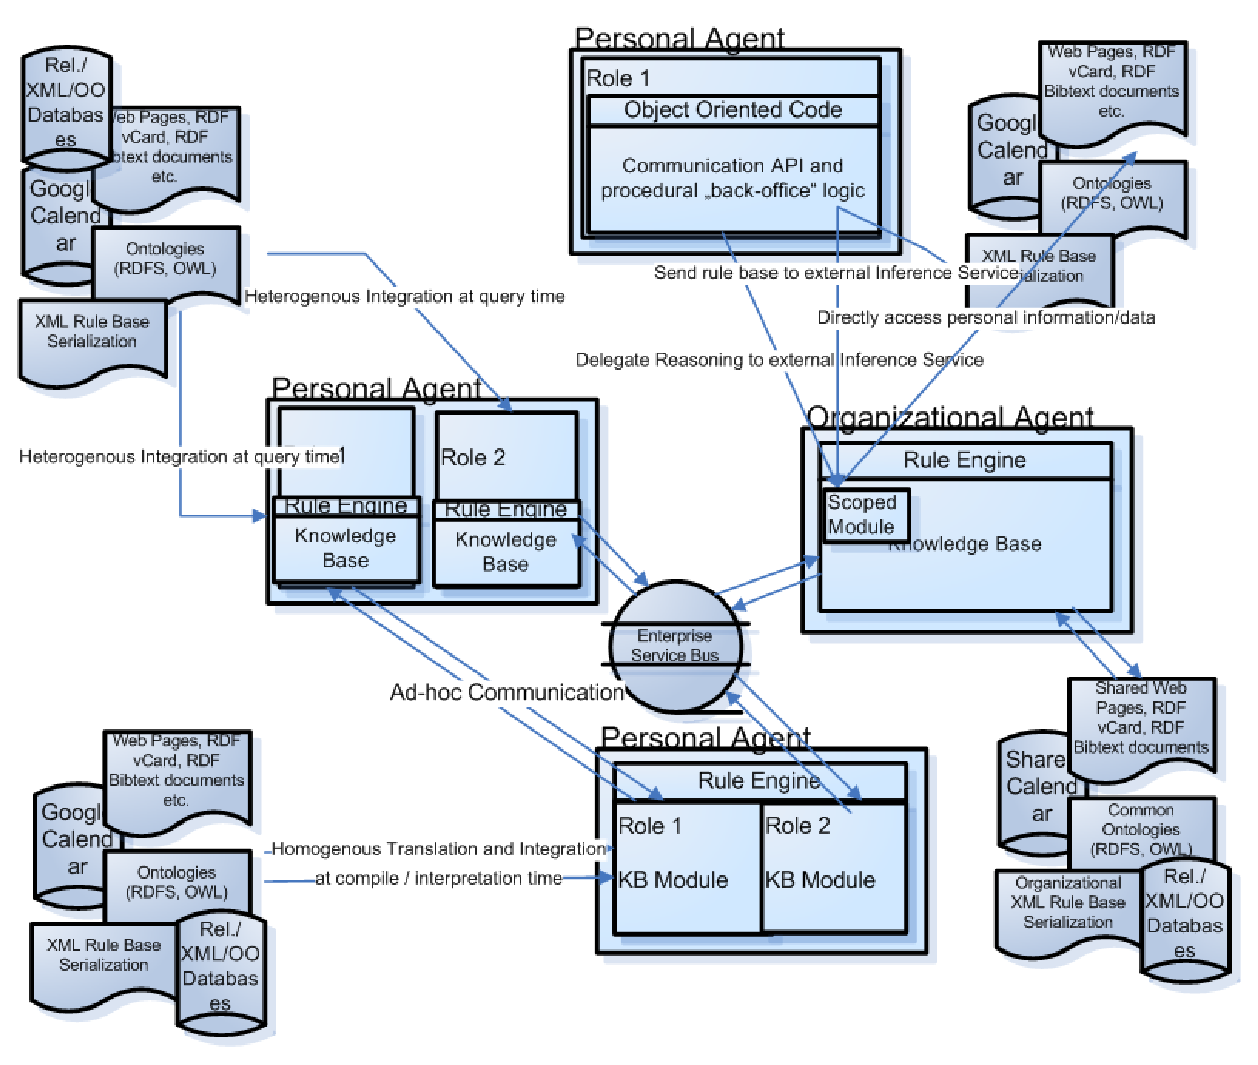
\includegraphics[scale=0.4]{img_rr01}
% \caption{Rule Responder Architecture, taken from \cite{2007-Paschke_etal-RuleResponder.pdf}}
% \end{center}
% \end{figure*}



\subsubsection{Prova}
Prova is a highly expressive rule language with a clear orientation towards CEP. It uses backward-reasoning logic to formalize decisions in terms of derivation. Forward-directed messaging of reaction rules supports distributed event and action processing. It is used by the authors of \cite{2013_Zhao-Paschke_EDSWE.pdf,2007-Paschke_etal-RuleResponder.pdf}. It allows dynamic access to external data sources.


\subsubsection{(Reaction) RuleML}
%\subsubsection{\textit{(Reaction) RuleML}}
\textit{RuleML}~\cite{2006-Boley-RuleML.pdf} is a XML-based rule specification standard to express both forward and backward rules for derivation, reaction, rewriting, messaging, verification and transformation. The building blocks of \textit{RuleML} are predicates, derivation rules, facts, queries, integrity constraints and transformation rules. Its development is driven by the Rule Markup Initiative~\cite{wwwruleml}.

With \textit{RuleML} being already a large specification, \textit{Reaction RuleML}~\cite{2012-Paschke_etal-ReactionRuleML.pdf} extends \textit{RuleML} towards reaction rules and complex event/action messages, e.g. for complex event processing (CEP). It adds various kinds of production, action, reaction and knowledge representation (KR) temporal/event/action logic rules, as well as (complex) event/action messages. It consists of one general reaction rule form that can be specialized, e.g. into production rules, trigger rules, ECA rules or messaging rules. Three different execution styles (active, messaging,  reasoning). Messages define inbound or outbound event messages and are used to interchange events and rule bases. A reaction rule can be globally or locally nested within other reaction or derivation rules. Additionally the RuleML Interface Description Language (\textit{RuleML IDL}) was provided, a sublanguage of \textit{Reaction RuleML} and allows the description of public rule functions as interfaces to hide program logic.

As research continued in terms of reaction rules and \textit{Rule Responder}, the authors of \cite{2013_Zhao-Paschke_EDSWE.pdf} showed the adoption of event paradigms to support scientific workflow execution. In their work they point out the limitation of ECA frameworks when adopted to their use case. For highly distributed and loosley coupled scientific workflows, complicated conditional procedures and rules, which can also have local scopes, are required. This shows us their work is going towards large systems with a highly developed rule language that subsumes research from several fields. 

OO jDrew~\cite{2005-Ball_etal-OOjDrew.pdf} is a Java based rule engine, capable of parsing and executing RuleML.

%\begin{lstlisting}[breaklines]
%<Rule>
%  [...]
%  <on>      </on>
%   <if>      </if>
%   <then>    </then>
%   <do>      </do>
%   <after>   </after>
%   <else>    </else>
%   <elsedo>  </elsedo>
% </Rule>

% \end{lstlisting}




\subsubsection{JSON Rules}
JSON Rules\cite{2008-Giurca_Pascalau-JSON_Rules.pdf} has been invented due to an increasing need for rules in terms of semantic web applications and the emerging Rich Internet Applications (RIAs). JSON rules is capable of expressing production rules (if-do) as well as ECA rules (on-if-do). The rules engine is a forward chaining rule engine using a modified RETE~\cite{1982-Crockford-RETE.pdf} algorithm. The RETE working memory in this rule engine is the (event-based) Document Object Model (DOM) itself. An example~\cite{2009-Pascalau_Giurca-RBACEM.pdf} of (DOM-)rule-based creation and execution of mashups illustrates the powerful aspects of JSON Rules.

\subsection{Mashups}
In \cite{2011-Pascalau-MBC.pdf}, one of the founders of JSON Rules proposes to look at mashups as user-behaviour in a certain context. A mashup, to achieve a user-defined goal, is modelled via Unified Modeling Language (UML) as a map containing contexts and behaviour desriptions. Contexts are defined as a set of concepts, concepts are defined as unit of knowledge created by unique combination of characteristics. A mashup is then defined as  set of contexts behaviour, where behaviour consists of rules and processes. The conceptual work done in this paper is interesting but the running example isn't accessible.

It is also important to understand what users expect from service mashups. In \cite{2010-Namoun_etal-EURCW.pdf} research is done in identifying user perceptions of services, their composition, user working ways and expectations towards a composition tool. They come up with a set of guidelines and recommendations to aid the development of mashup environments. A survey~\cite{2009-Fischer_etal-OCAMG.pdf} that went into a similar direction categorizes the different frameworks for user driven mashup development as based on:
 \begin{itemize}
%\itemsep-1.5em
  \item Programming Paradigm
  \item Scripting Languages
  \item Spreadsheets
  \item Wiring Paradigm
  \item Programming by Demonstration
  \item Automatic Creation of Mashups
\end{itemize}
But even though large efforts are made in all these research fields, unexperienced users are still not able to build mashups without knowledge about numerous aspects of the framework or programming.

\subsubsection{useKit}
The idea of useKit~\cite{2010-Rizzotti_Burkhart-useKit.pdf} missions shows us the potential of user-defined cloud application mashups. While their approach is not event-based, it can be regarded as an evolution base for the web towards reactive cloud application mashups.

\subsubsection{Rule Responder}
Rule Responder~\cite{2007-Paschke_etal-RuleResponder.pdf} is a project to extend the Semantic Web towards a Pragmatic Web infrastructure for collaborative human-computer networks, which they call an architecture of a Pragmatic Agent Web (PAW). It supports the formation of virtual groupings and allows semi-automated agents with their individual contexts, decisions and actions. The authors postulate agents empowered with automatic rule-driven data transformation, decision derivation from existing knowledge and reaction according to changed situations or occurred events. The work done in this project concentrates on a layer on top of a rule engine and language, and thus allows for a combination of arbitrary rule-based systems via their framework. This is achieved through the usage of general messge oriented communication interfaces and a platform-independent rule interchange format.

The authors of Rule Responder built their reference system\cite{wwwruleresponder} on top of the Mule~\cite{wwwmuleesb} open-source Enterprise Service Bus (ESB) which acts as a communication middleware. The decision to use Mule was made because it goes beyond the typical definition of an ESB by providing a distributable object broker to manage all sorts of service components. Each agent runs its own rbitrary rule engine. For demonstartion purposes Prova and OO jDrew were used to demonstrate the rule interchange between different rule engines.

\subsubsection{DashMash}
The DashMash~\cite{2011-Cappiello_etal-DashMash.pdf} platform is an approach to give end-users the graphical tools in a browser to mash up web applications in a dashboard. A resource of (for stability reasons) trimmed services (such as GoogleMaps or TripAdvisor), filters, viewers and generic components is accessible to the users. DashMash uses an event-driven model of the presentation level, similar to a JSON Rules approach in \cite{2009-Pascalau_Giurca-RBACEM.pdf}. Events sent by the client to the server are used to update all viewers with the actual data the user is looking at.

\section{Use Case Study}
In order to verify some of the identified related work, use cases around the succcessor of useKit~\cite{2010-Rizzotti_Burkhart-useKit.pdf} (ProBinder~\cite{wwwprobinder}) have been derived and investigated. 

\subsection{Binder Watcher}
Binder Watcher is about binders being watched and actions that are taken after certain changes to a binder. Users of ProBinder, which are involved in many different companies and project binders, tend to be confronted with a large amount of information. It is a tedious task to get the user's context back into a clean state, where the ProBinder system is ready to reflect new recent changes in an optimal way to the user. By allowing the users to identify resources (binder tabs in this case, but could also be complete binders, persons, companies, \dots) of interest, the user task can be automated to a certain extent. As soon as changes are made to the resources of interest, they are marked as read and summarized. These summaries are then provided to the user, which allows him to identify the most important changes.

The Binder Watcher use case was implemented in KRL (see \ref{app:uc_bw_krl}) and provided the important insight that the realization of such a use case in an ECA is a time-consuming challange. 

\subsection{Web Watcher}

\subsection{Calendar Manager}


\section{Conclusion}
What did we look at
How is the evolving of the web possible with these approaches
how are we going to make it reactive
where does the reactiveness happen
interchangeable events important, rules not so much?
we only need events communicated and the communiation between them doesn't happen via a clumsy bus.
mashups?


flexibility and agility of the solution granted by interchangable rules, do we really need this?
are we not more going towards a system which consumes events and has user defined rules.
there the rules come into play and of course it would be nice to have them in a Reaction RuleML style.
let users write rules in  RuleMl in a first stage, then simplify the vocabulariy as good as possible.
instead of weaving stubs or proxies of existing service into a message oriented middleware (MoM), the web itself is used as the MoM. Through this a lightweighted and performant event-based architecture can be realized, which allows the orchestration of existing web and cloud applications.

a choreography is when an agent forms a collaboration with another one in order to fulfill the task.


In \cite{2009-Pascalau_Giurca-LWAECARE.pdf}, the founders of JSON Rules~\cite{2008-Giurca_Pascalau-JSON_Rules.pdf} describe a lightweight architecture that allows to react and proact on behalf of events in the ontology of web browsers.
JSON Rules seems to be very promising for our work because of its leightweight architecture and specialization on production and ECA rules. But the existing working memory architecture needs to be generalized to allow a different environment, other than just the DOM tree. The existing architecture could be used to allow the user to create local rules that do not access remote systems and thus runs into authentication issues.

Data flow instead of event flow, no reactivity.
Under related work, \cite{2010-Namoun_etal-EURCW.pdf} pointed out the difficulties of unexperienced users to tackle the execution flow. This issue arose from their approach of displaying all services as very similar UI's. Adopting an event-based system, where event producers are clearly different from action consumers would address this issue in an intuitive way.

\section{Future Work}

Developing an ECA architecture which promotes cloud applications as event-based first-class citizens and allows for an intuitive user-driven mashup development is a research field that has, to the best of our knowledge, not been addressed yet. Looking at cloud-based applications as event producers and action consumers gives new ways to bring reactivity into the existing web. Such representations require a rule-based system that allows their interweaving. Not solely the interaction between cloud applications should be addressed, but also with the browser itself, since it is a tool which is prdominantly used to access the web. This would empower the user to predefine influences and interactions on existing cloud applications before they are accessed.

Since the vision of on- and offline rules can't be covered with a single server application, the utilization of a fast, flexible and widely used technology such as JavaScript to tackle this challange seems to be favorable future work. JavaScript was mainly invented for browsers and is spread all over the web by now. Additionally, applications such as Node.js~\cite{wwwnodejs}, bring JavaScript to the server-side and tear down the communication efforts between cloud applications through JSON messages which are directly understood by modern browsers and cloud applications.
Preferably a lightweighted rules engine would be used to run the user-generated mashups. The KRE suits the demand for a certain coupling between the users browser and the remote rules engine to provide a powerful system. On the other hand the rules engine is not (yet) well documented, nit lightweighted and forged in Perl, a programming language that wasn't encountered during the research for related work on rule based systems.

Sharing and thus exchanging of rules gives new ways for collaboration and the possibility for expert users to aid less experienced ones, giving them the chance to catch up. 
In terms of usability an easy to understand way to create rules would have a large benefit. We envision a graphical toolkit that empowers users to build their own complex event-based cloud application mashups, powerful RIAs.

It is interesting, that all related work we looked at, only used public cloud applications, thus omitting the challenge of authorization and security of the user's private context.
If users are provided the tools to access public cloud APIs and create mashups with them, they are going to benefit from this. But mostly users these days are travelling in the web within their private, secured context. Thus the access to such resources are providing even more power- and meaningful tools to the user. 

\bibliography{liveweb}
\bibliographystyle{related-work}

\newpage
\appendix
\renewcommand\thesection{Appendix \Alph{section}}

\section{Binder Watcher KRL code} \label{app:uc_bw_krl}
\begin{lstlisting}[breaklines]
ruleset a2236x4 {
  meta {
  	name "ProBinder Flag Notification Handler"
  	description "This is a first example on how to react on ProBinder Events"
  	author "dominic.bosch"
    //ProBinder IDs:
    // userID: 10595
    // companyID: 643
    // contextID: 16694
    // followerID: 12613
    
  	logging on
  }
  
  dispatch {}
  
  global {}
  
  // Reset all entitiy variables
  rule resetAll {
    select when probinder resetall
      send_directive("Full Reset");
      fired {
        clear ent:userID;
        clear ent:companyID;
        clear ent:contextID;
        clear ent:credentials;
        clear ent:followers;
        clear ent:newContents;
        clear ent:summary;
        clear ent:temp;
      }
  }
  
  // reset the unread content data structures
  rule reset {
    select when probinder reset
      send_directive("Reset, user credentials and followers still kept");
      fired {
        clear ent:newContents;
        clear ent:summary;
        clear ent:temp;
      }
  }
  
  // The user registers himself with email and password for the ProBinder API...
  rule register_user {
    select when probinder register
      if (event:attr('userID').as("str") neq 'null'
          && event:attr('companyID').as("str") neq 'null'
          && event:attr('contextID').as("str") neq 'null'
          && event:attr('email').as("str") neq 'null'
          && event:attr('password').as("str") neq 'null') then {
        send_directive("user registered");
      }
      fired {
        set ent:userID event:attr('userID');
        set ent:companyID event:attr('companyID');
        set ent:contextID event:attr('contextID');
        set ent:credentials uri:escape(event:attr('email')) + ":" + uri:escape(event:attr('password'));
      }
  }
  
  // The user sent an event that tells us he wants to follow somebody
  rule new_user_to_follow {
    select when probinder newfollower
      pre{
        listFollowers = ent:followers || {};
        newfollower = event:attr('followerID').as("str");
        listFollowers = listFollowers.put([newfollower], "true");
      }
      if (event:attr('userID') == ent:userID
          && newfollower neq "null") then {
            send_directive("New ProBinder User added to followers");
      }
      fired{
        set ent:followers listFollowers
      }
  }
  
  // Let the KRE check ProBinder for new unread content and process it immediately
  rule check_for_unread_content {
    select when probinder check
      pre {
        r = http:get("https://" + ent:credentials + "@probinder.com/service/36/unreadcontent");
        arr = r{"content"}.decode();
      }
      send_directive("Checked ProBinder for unread content, found: " + arr.length());
      fired {
        set ent:newContents arr;
        raise explicit event processnewcontents;
      }
    
  }
  
  // Work (new unread content) from ProBinder to process
  rule process_new_contents {
    select when explicit processnewcontents
    // Process only the unread contents from people we are following,
    // filter condition omits unnecessary rules invocation
    foreach ent:newContents.filter(
      function(d) {ent:followers.pick("$."+d.pick("$.userId")) != null}
    ) setting(nc)
      pre {
        s = ent:summary || {};
        cid = nc.pick("$.id");
        r = http:get("https://" + ent:credentials
          + "@probinder.com/service/2/get?id=" + cid
          + "&service=" + nc.pick("$.serviceId"));
        arr = r{"content"}.decode();
        
        userid = arr.pick("$.userId");
        storeKey = arr.pick("$.lastModified");
        truncStr = arr.pick("$.text");//.extract(re/^.{100}/gi); // should shorten the text...
        
      //TODO Process different kind of unread contents differently
        str = {"content": truncStr}; //[0]
        s = s.put([userid, storeKey], str);
      }
      http:get("https://" + ent:credentials + "@probinder.com/service/2/setread?id=" + cid);
      always {
        set ent:summary s;
      }
    
  }
  
  rule send_summary{
    select when probinder heartbeat
    always {
      clear ent:temp;
      raise explicit event filltemp;
    }
  }
  
  rule fill_temp{
    select when explicit filltemp
    always {
      set ent:temp ent:summary;
      raise explicit event mergecontent;
    }
  }
  
  // When somebody sends a periodic heartbeat, this summary is produced
  // The periodic invocation of this rule might be possible to implement in the KRE
  rule merge_content {
    select when explicit mergecontent
    foreach ent:temp setting (userID)
      pre {
        s = ent:temp;
        userBulk = s.pick("$."+userID);
        sumry = userBulk.pick("$..content").join(" ");
      }
      http:get("https://" + ent:credentials + "@probinder.com/service/27/save?companyId="
        + ent:companyID + "&context=" + ent:contextID + "&text=test");
      send_directive("Stored summary in your predefined binder:" + sumry);

  }
  
  rule print_summary {
    select when probinder printsum
      send_directive(ent:summary);
  }
}
\end{lstlisting}

\end{document}
